% ===========================================================================
% 05_estado_actual.tex — Estado del proyecto al 27 de julio de 2026.
%
% Esta secci\'on reemplaza la lectura optimista de la secci\'on 03 con lo que
% realmente qued\'o en pie, y a\~nade el resultado que cierra el \'ultimo hueco
% experimental: la inflaci\'on no es de NUESTRO modelo, es del protocolo.
%
% Todas las cifras salen de artefactos versionados bajo results/comparison/.
% Las figuras las genera analysis/make_slide_figures.py desde esos mismos
% archivos: si un n\'umero cambia, se regenera la figura, no se edita a mano.
%
% Trabajos SLURM citados: 5761-5768 y 5816-5823 (protocolo transductivo,
% 4 semillas), 5808-5844 (rejilla multi-semilla), 5827 (piso topol\'ogico),
% 5849-5852 (rejilla entre arquitecturas).
% ===========================================================================

\section{Estado actual (julio 2026)}

% ---------------------------------------------------------------------------
\begin{frame}{\textquestiondown{}Qu\'e cambi\'o desde la defensa?}
  \begin{block}{Tres cosas, en orden de importancia}
    \small
    \begin{enumerate}
      \item<1-> \textbf{Se arreglaron dos errores en la construcci\'on del grafo} y se
            volvi\'o a medir todo sobre el grafo corregido, con 4 semillas en vez de una.
            \emph{El resultado se replica.}
      \item<2-> \textbf{El proyecto ya no afirma nada sobre esclerosis m\'ultiple.} La
            etiqueta de enfermedad nunca entra al modelo: ni como variable, ni como
            objetivo, ni como entrada de ninguna cabeza. Pasa a ser \emph{procedencia
            de los datos}.
      \item<3-> \textbf{La inflaci\'on que reportamos no es un defecto de nuestro modelo:
            es del protocolo de evaluaci\'on.} Es el resultado nuevo, y es el que
            convierte esto en un art\'iculo de m\'etodos.
    \end{enumerate}
  \end{block}

  \onslide<3->{%
  \begin{block}{Lectura}
    \scriptsize
    Los puntos 1 y 2 protegen el trabajo de una cr\'itica. El punto 3 es lo que le da
    un aporte propio. Las siguientes diapositivas explican el 3 paso a paso.
  \end{block}}
\end{frame}

% ---------------------------------------------------------------------------
\begin{frame}{El problema, en una frase}
  \begin{block}{La objeci\'on que cualquier revisor iba a hacer}
    \small
    \emph{``Ustedes solo demostraron que \textbf{su} modelo estaba mal evaluado.
    Eso es un reporte de error en su c\'odigo, no un hallazgo sobre el campo.''}
  \end{block}

  \vspace{0.3em}
  \onslide<2->{%
  \begin{block}{Y ten\'ia raz\'on}
    \small
    Todo lo medido hasta ahora era \textbf{una sola arquitectura}: la nuestra.
  \end{block}}

  \vspace{0.3em}
  \onslide<3->{%
  \begin{block}{La respuesta}
    \small
    Correr \textbf{seis arquitecturas} por los \textbf{dos protocolos}. Si la inflaci\'on
    aparece en todas --- incluso en una que \textbf{no ve el grafo} --- entonces no puede
    ser una propiedad del transformer.
  \end{block}}
\end{frame}

% ---------------------------------------------------------------------------
\begin{frame}{El dise\~no: dos decisiones, cuatro casillas}
  \small
  Un experimento de predicci\'on de enlaces se puede inflar por \textbf{dos v\'ias
  independientes}. Las cruzamos.

  \vspace{0.5em}
  \begin{columns}[T]
    \begin{column}{0.52\textwidth}
      \begin{itemize}
        \item<1-> \textbf{(a) Qu\'e aristas se prueban.} Si las aristas de prueba
              tambi\'en estaban en entrenamiento, se mide \emph{memoria}, no predicci\'on.
        \item<2-> \textbf{(b) C\'omo se eligen los pares falsos.} Al azar caen casi
              siempre en genes impopulares: entonces ``\textquestiondown{}es real?''
              se vuelve ``\textquestiondown{}es popular este gen?'', que no necesita
              biolog\'ia.
      \end{itemize}
      \vspace{0.4em}
      \onslide<3->{\scriptsize Dos decisiones binarias $\Rightarrow$ \textbf{cuatro
      casillas}. En cada una se entrenan las seis arquitecturas.}
    \end{column}

    \begin{column}{0.46\textwidth}
      \centering
      \begin{tikzpicture}[scale=0.92, every node/.style={font=\scriptsize}]
        % Ejes. Sin t\'itulo rotado en el eje Y: chocaba con las etiquetas de fila, as\'i
        % que las filas se nombran solas.
        \node[align=center, text=msgray] at (1.5,3.15) {controles falsos};
        \node[align=center] at (0.75,2.62) {al azar};
        \node[align=center] at (2.25,2.62) {pareados};
        \node[align=right, anchor=east] at (-0.15,1.85) {aristas\\\textbf{vistas}};
        \node[align=right, anchor=east] at (-0.15,0.65) {aristas\\\textbf{retenidas}};

        % casilla 1 — el protocolo original
        \onslide<1->{%
          \fill[msorange!22] (0.05,1.30) rectangle (1.45,2.40);
          \node[align=center] at (0.75,1.85) {protocolo\\\textbf{original}};}
        % casilla 2 — solo negativos honestos
        \onslide<2->{%
          \fill[mslight] (1.55,1.30) rectangle (2.95,2.40);
          \node[align=center] at (2.25,1.85) {solo (b)\\arreglado};}
        % casilla 3 — solo split honesto
        \onslide<2->{%
          \fill[mslight] (0.05,0.10) rectangle (1.45,1.20);
          \node[align=center] at (0.75,0.65) {solo (a)\\arreglado};}
        % casilla 4 — el protocolo honesto
        \onslide<3->{%
          \fill[mscyan!30] (1.55,0.10) rectangle (2.95,1.20);
          \node[align=center] at (2.25,0.65) {protocolo\\\textbf{honesto}};}

        \onslide<3->{%
          \draw[->, very thick, msorange] (1.15,1.72) -- (1.95,0.82);}
      \end{tikzpicture}
    \end{column}
  \end{columns}

  \vspace{0.4em}
  \onslide<3->{%
  \begin{block}{Detalle que importa}
    \scriptsize
    Dentro de cada casilla, cada modelo se puntu\'a con \textbf{ambos} muestreadores de
    negativos, y siempre se reportan casillas donde entrenamiento y evaluaci\'on
    \textbf{coinciden}. Mezclarlos mide el desajuste, no la dificultad --- es la trampa
    que documentamos en la secci\'on anterior.
  \end{block}}
\end{frame}

% ---------------------------------------------------------------------------
\begin{frame}{Las cuatro casillas, para el HGT}
  \centering
  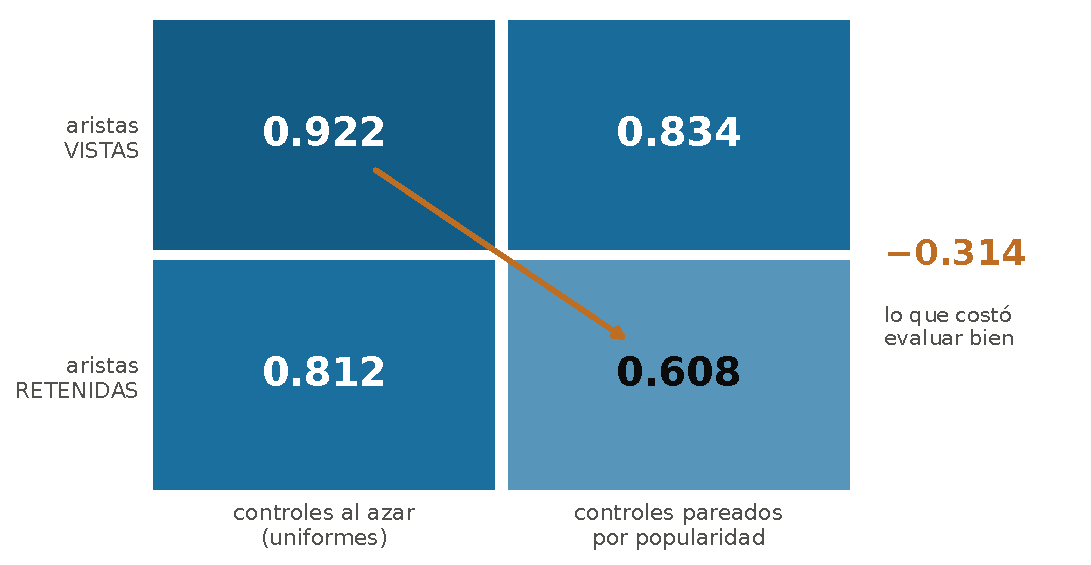
\includegraphics[width=0.62\textwidth]{../../results/figures/slides_02_rejilla_protocolo.pdf}

  \vspace{0.1em}
  \raggedright
  \begin{block}{Lectura}
    \scriptsize
    Arriba-izquierda es el protocolo de la defensa; abajo-derecha el honesto. Entre ambos
    hay \textbf{0.314 de AUROC} que no eran del modelo, sino de c\'omo se med\'ia.
    \onslide<2->{\textbf{Arreglar solo una de las dos v\'ias no alcanza:} las casillas
    intermedias (0.834 y 0.812) siguen muy por encima de 0.608 --- el da\~no es
    \textbf{super-aditivo}, as\'i que retener aristas pero conservar controles al azar
    sigue dando un n\'umero inflado.}
  \end{block}
\end{frame}

% ---------------------------------------------------------------------------
\begin{frame}{El mecanismo, atrapado en el acto}
  \scriptsize
  Mismo modelo, mismas aristas retenidas: \textbf{solo cambian los pares falsos al
  evaluar.}

  \vspace{0.1em}
  \centering
  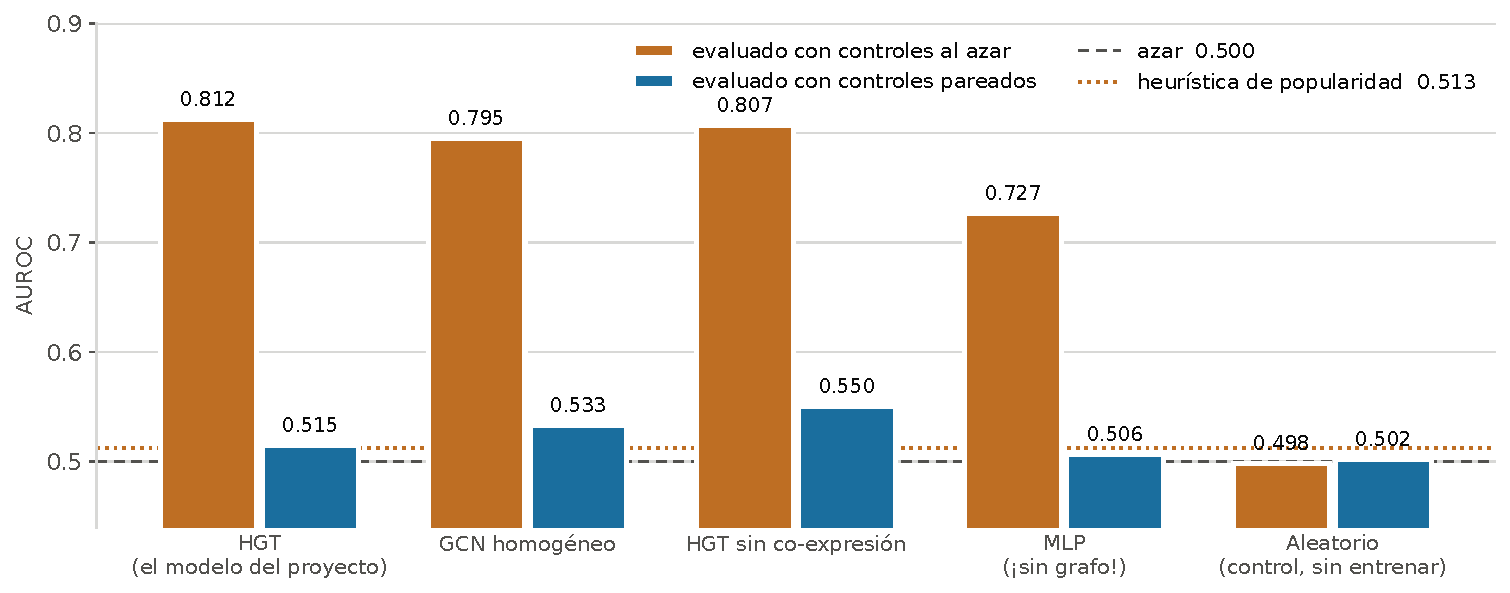
\includegraphics[width=0.80\textwidth]{../../results/figures/slides_03_colapso_negativos.pdf}

  \vspace{0.1em}
  \raggedright
  \begin{block}{Lectura}
    \scriptsize
    Todo modelo entrenado con controles al azar \textbf{se derrumba al azar} en cuanto se
    parean por popularidad: aprendi\'o popularidad del gen, no regulaci\'on.
    \onslide<2->{\textbf{El control aleatorio no se mueve} (0.498 $\to$ 0.502) --- eso es
    lo que vuelve cre\'ible al resto: el efecto no lo fabrica nuestro c\'odigo.}
  \end{block}
\end{frame}

% ---------------------------------------------------------------------------
\begin{frame}{El resultado que cierra el hueco}
  \centering
  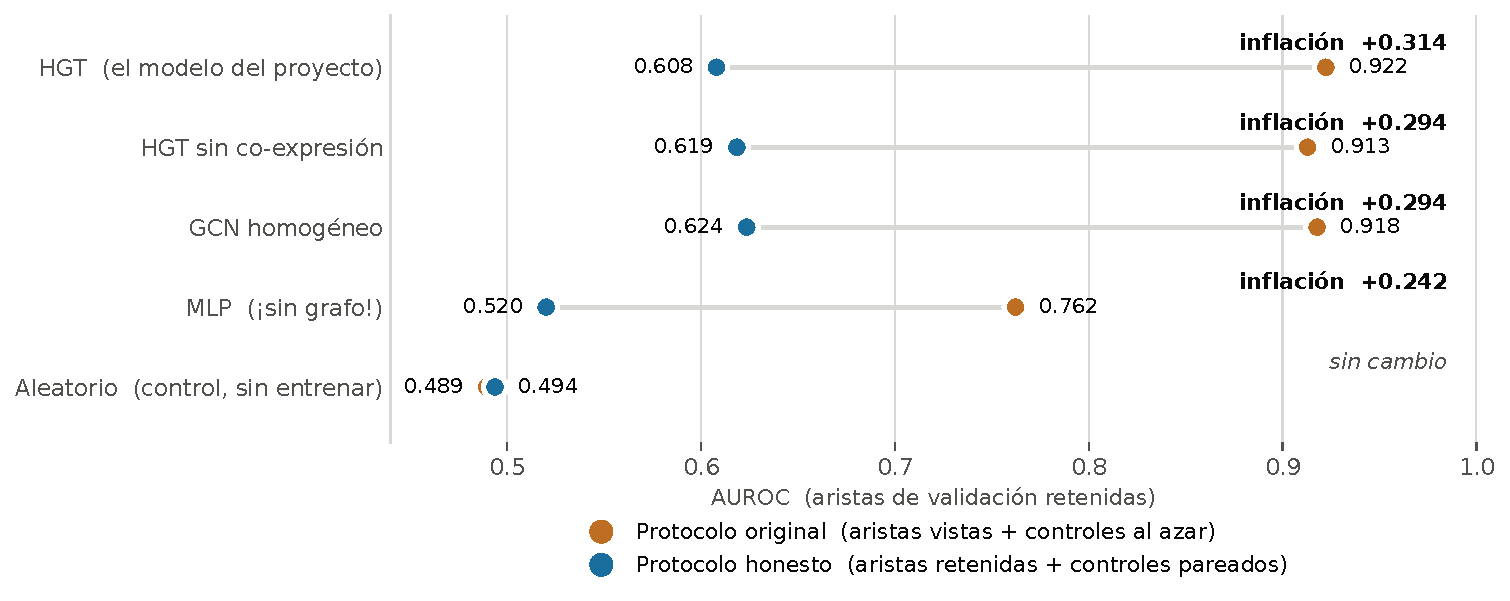
\includegraphics[width=0.84\textwidth]{../../results/figures/slides_01_inflacion_por_arquitectura.pdf}

  \vspace{0.1em}
  \raggedright
  \onslide<2->{%
  \begin{block}{Lectura}
    \scriptsize
    \textbf{Todas las arquitecturas entrenadas se inflan entre 0.24 y 0.31} --- incluido un
    MLP que \textbf{no ve el grafo en absoluto}. El control sin entrenar no se mueve. La
    inflaci\'on no es del transformer, ni del paso de mensajes heterog\'eneo, ni siquiera
    de \emph{tener} un grafo: es \textbf{del protocolo}. Es la afirmaci\'on sobre la que se
    sostiene el art\'iculo, y ahora est\'a medida, no argumentada.
  \end{block}}
\end{frame}

% ---------------------------------------------------------------------------
\begin{frame}{Dos hallazgos que no ten\'iamos}
  \begin{block}{1. El MLP explica el mecanismo}
    \small
    La super-aditividad se replica en \textbf{todos} los modelos con grafo. El MLP es la
    excepci\'on \emph{informativa}: sin grafo, su \'unica se\~nal disponible \textbf{es} el
    grado del gen, as\'i que la v\'ia de los negativos absorbe casi todo el da\~no
    ($-0.263$).

    \vspace{0.2em}
    \onslide<2->{Su casilla ``aristas vistas + controles pareados'' da \textbf{0.4994}:
    azar exacto. \emph{Se le permite memorizar las respuestas y a\'un as\'i no le gana a
    una moneda al aire}, porque los controles pareados le quitan lo \'unico que sab\'ia
    hacer.}
  \end{block}

  \vspace{0.2em}
  \onslide<3->{%
  \begin{block}{2. El GCN simple le gana al transformer}
    \small
    En el protocolo honesto: \textbf{GCN homog\'eneo 0.6236} frente a \textbf{HGT 0.6080}.
    La arquitectura heterog\'enea de 4 capas y 512 canales \textbf{no est\'a pagando su
    costo} ni siquiera contra la l\'inea base m\'as simple con grafo.

    \vspace{0.2em}
    Y el MLP (0.5202) \emph{pierde} contra Adamic--Adar (0.5912): el grafo es
    \textbf{necesario} para superar el piso topol\'ogico, solo que no alcanza para
    superarlo por mucho.
  \end{block}}
\end{frame}

% ---------------------------------------------------------------------------
\begin{frame}{Lo que s\'i se sostiene, sobre el grafo corregido}
  \small
  Reentrenado y reevaluado con \textbf{4 semillas} sobre \texttt{graphs\_v3fixed}
  (verificado de forma independiente):

  \vspace{0.4em}
  \centering
  \begin{tabular}{lc}
    \toprule
    \textbf{Medici\'on (conjunto de prueba)} & \textbf{AUROC} \\
    \midrule
    Protocolo original (aristas vistas, controles al azar) & 0.9867 $\pm$ 0.0011 \\
    \textbf{Protocolo honesto} (retenidas, pareados) & \textbf{0.6276 $\pm$ 0.0070} \\
    Mejor heur\'istica \emph{sin aprendizaje} (\texttt{adamic\_adar}) & 0.5912 \\
    \midrule
    Clasificaci\'on de tipo celular --- \emph{intacta y real} & \textbf{0.9916} \\
    Mejor control \emph{sin grafo} (\texttt{logistic\_regression} sobre \texttt{X\_pca}) & 0.6692 \\
    \bottomrule
  \end{tabular}

  \vspace{0.5em}
  \raggedright
  \begin{block}{Lectura}
    \scriptsize
    \textbf{Todo se replica.} El 0.6271 de una sola semilla sobre el grafo anterior queda
    dentro de 0.1$\sigma$ del 0.6276 de cuatro semillas sobre el grafo corregido, y el
    da\~no total ($-0.3591$) reproduce el anterior ($-0.357$) con 0.002 de diferencia.

    \vspace{0.2em}
    \onslide<2->{Que un resultado sobreviva \textbf{a cambiar el grafo y repetir el
    experimento} es evidencia de que describe el protocolo, no un grafo con errores.
    El piso topol\'ogico (0.5912) sali\'o \emph{id\'entico}: los arreglos nunca tocaron la
    topolog\'ia miRNA$\to$gen.}

    \vspace{0.2em}
    \onslide<3->{La clasificaci\'on celular ya tiene su propio control sin aprendizaje
    (job 5853, 2026-07-29): 32 puntos de brecha con \texttt{X\_pca} solo, sin pasar
    mensajes por el grafo --- muy por encima de los 3.6 puntos de \texttt{adamic\_adar}.
    \textbf{No es circular} aunque la etiqueta sea \texttt{argmax(marker score)} por
    construcci\'on (coincide en 100\% de las c\'elulas): el modelo nunca ve esos scores,
    solo \texttt{X\_pca} y el grafo, y aun as\'i el control sin grafo se queda muy corto.}
  \end{block}
\end{frame}

% ---------------------------------------------------------------------------
\begin{frame}{Honestidad sobre estos n\'umeros}
  \begin{block}{Dos advertencias que viajan con la tabla anterior}
    \small
    \begin{itemize}
      \item<1-> \textbf{La rejilla entre arquitecturas es $n=1$} (semilla 42), a
            prop\'osito. La inflaci\'on es de 0.24--0.31 y la dispersi\'on entre semillas,
            donde s\'i pudimos medirla, es de 0.005--0.02: el efecto es mucho mayor que el
            ruido. \emph{Se reporta como $n=1$ y sin barra de error.}
      \item<2-> \textbf{El HGT aparece con 0.6080 aqu\'i y con 0.6276 en la tabla
            anterior.} Misma arquitectura y mismo criterio de selecci\'on, pero
            \texttt{run\_baselines.py} entrena con su propio bucle de una sola GPU y queda
            0.02--0.06 m\'as bajo. Esa tabla sirve para \textbf{comparar arquitecturas
            entre s\'i} en condiciones id\'enticas, no para repetir el titular.
    \end{itemize}
  \end{block}

  \vspace{0.2em}
  \onslide<3->{%
  \begin{block}{Y un detalle que probablemente merece estar en la discusi\'on}
    \scriptsize
    El criterio de selecci\'on por \texttt{val\_loss} ya se hab\'ia identificado y
    corregido en \texttt{train.py} --- ah\'i est\'a documentado que guardaba un modelo al
    azar (0.5324) para uno que alcanza 0.6268. \textbf{El arreglo nunca lleg\'o a
    \texttt{run\_baselines.py}}, y se detect\'o por un s\'intoma (paro temprano en la
    \'epoca 29 en vez de 124) con la rejilla ya corriendo: hubo que cancelarla y repetirla.

    \vspace{0.2em}
    Es decir: \emph{nuestra propia herramienta de auditor\'ia carg\'o exactamente el tipo
    de error que este art\'iculo denuncia.} Vale m\'as decirlo que un p\'arrafo gen\'erico
    de limitaciones.
  \end{block}}
\end{frame}

% ---------------------------------------------------------------------------
\begin{frame}{\textquestiondown{}D\'onde estamos para publicar?}
  \begin{block}{Ya no falta medir nada para la afirmaci\'on central}
    \small
    El \'ultimo hueco experimental se cerr\'o. Lo que queda \textbf{no requiere GPU}:
    \begin{itemize}
      \item<2-> \textbf{Tres decisiones} de redacci\'on: \textquestiondown{}el
            ``ciego a la enfermedad'' es aporte o limitaci\'on?; \textquestiondown{}se
            publica el hallazgo de que 37 pacientes de T1D estaban archivados como
            controles sanos?; \textquestiondown{}lo lleva tambi\'en el resumen para
            colaboradores?
      \item<3-> \textbf{Alcance:} ampliar la revisi\'on de literatura (piloto $n=7$) y
            correr los brazos de miRTarBase --- \emph{ya descargados y pre-registrados}.
      \item<4-> \textbf{Trabajo de manuscrito:} retitular, corregir la procedencia de los
            datos, autor\'ia, y elegir una revista de \textbf{evaluaci\'on/m\'etodos}.
    \end{itemize}
  \end{block}

  \vspace{0.2em}
  \onslide<5->{%
  \begin{block}{\textquestiondown{}Hacen falta m\'as datos? \textbf{No}}
    \scriptsize
    M\'as c\'elulas no toca el cuello de botella (la clasificaci\'on celular ya est\'a en
    0.9916). M\'as muestras de miRNA tampoco: las \textbf{166 que ya tenemos} no las lee
    ning\'un modelo. Y a\~nadir secuencia es \textbf{circular} mientras el objetivo sea
    miRDB, que \emph{es} un modelo de complementariedad de semilla.

    \vspace{0.2em}
    Lo \'unico que a\~nadir\'ia algo --- miRTarBase como segunda fuente independiente ---
    \textbf{ya est\'a en disco}. No es un problema de datos: es de escritura.
  \end{block}}
\end{frame}

% ---------------------------------------------------------------------------
% Marco de cierre a\~nadido el 2026-07-27. El deck termina donde empez\'o: con la
% respuesta a ``\textquestiondown{}aportamos algo?'' --- pero ahora respaldada por
% todo lo que va en medio. Es el espejo del marco de la secci\'on 1.
% ---------------------------------------------------------------------------
\begin{frame}{Cerrando: \textquestiondown{}aportamos algo?}
  \begin{block}{S\'i --- y conviene decirlo en una frase}
    \small
    \emph{La evaluaci\'on transductiva y los controles no pareados inflan la predicci\'on de
    blancos de miRNA en $\approx$0.36 de AUROC sobre un grafo biom\'edico real; la
    inflaci\'on aparece en \textbf{todas} las arquitecturas probadas ---
    \textbf{incluida una sin grafo} --- y no en el control sin entrenar; y una
    heur\'istica de una l\'inea que ignora al miRNA le gana a todas ellas bajo el protocolo
    de uso com\'un.\footnotemark}
  \end{block}
  \footnotetext{\tiny No es una afirmaci\'on aislada --- precedente externo verificado en
  las dos \'ultimas diapositivas.}

  \vspace{0.3em}
  \begin{columns}[T]
    \begin{column}{0.49\textwidth}
      \onslide<2->{%
      \begin{block}{Lo que dejamos utilizable}
        \scriptsize
        \begin{itemize}
          \item Un protocolo corregido con \textbf{prueba autom\'atica de fuga} ---
                reutilizable en cualquier grafo de interacciones.
          \item Tres controles sin aprendizaje y la rejilla de atribuci\'on 2$\times$2.
          \item Una lista de verificaci\'on para \textbf{claims espec\'ificos de contexto}
                (\textquestiondown{}est\'a la variable?, \textquestiondown{}la recibe el
                cabezal?, \textquestiondown{}var\'ia la evaluaci\'on con ella?).
          \item Un clasificador celular que \textbf{s\'i} funciona: 0.9916.
        \end{itemize}
      \end{block}}
    \end{column}
    \begin{column}{0.49\textwidth}
      \onslide<3->{%
      \begin{block}{Lo que \emph{no} aportamos, dicho sin rodeos}
        \scriptsize
        No hay descubrimiento de circuitos de regulaci\'on de miRNAs. No hay resultado
        espec\'ifico de tipo celular --- la arquitectura no pod\'ia producirlo. Y no hay
        una afirmaci\'on sobre esclerosis m\'ultiple: la etiqueta nunca entr\'o al modelo.

        \vspace{0.25em}
        \textbf{Es un art\'iculo de m\'etodos, no de biolog\'ia.} Y es defendible
        precisamente porque cada cifra de arriba est\'a medida, replicada y trazable a un
        artefacto.
      \end{block}}
    \end{column}
  \end{columns}
\end{frame}

% ---------------------------------------------------------------------------
% A\~nadida el 2026-07-29 para respaldar la frase "protocolo de uso com\'un" del cierre
% con precedente externo verificado, no solo con nuestro propio piloto de
% LITERATURE_SURVEY.md. Duplica la lista de results/EVALUATION_AUDIT.md \S"External
% precedent for these pitfalls" para que quede visible tambi\'en en el deck.
% ---------------------------------------------------------------------------
\begin{frame}{Referencias (1/2): fuga por aristas vistas}
  \small
  \begin{block}{(a) Fuga por aristas vistas / evaluaci\'on transductiva}
    \scriptsize
    \begin{itemize}
      \item \textbf{Toutanova \& Chen (2015).} \emph{Observed versus Latent Features for
            Knowledge Base and Text Inference.} CVSC Workshop, ACL 2015. --- el precedente
            can\'onico: WN18/FB15k se resuelven por relaciones inversas filtradas; por eso
            existe FB15k-237.
      \item \textbf{Zhu et al. (2023).} \emph{Pitfalls in Link Prediction with Graph Neural
            Networks.} arXiv:2306.00899. --- nombra exactamente nuestro problema
            (\emph{implicit test leakage}) y propone un arreglo.
      \item \textbf{Li, Shomer et al. (2023).} \emph{Evaluating GNNs for Link Prediction:
            Current Pitfalls and New Benchmarking.} NeurIPS 2023 (D\&B track),
            arXiv:2306.10453.
    \end{itemize}
  \end{block}

  \vspace{0.4em}
  \onslide<2->{%
  \begin{block}{Con cautela}
    \scriptsize
    Shchur et al. (2018, \emph{Pitfalls of GNN Evaluation}, arXiv:1811.05868) es real pero
    trata clasificaci\'on de nodos, no predicci\'on de enlaces: solo evidencia de que
    ``pitfalls de evaluaci\'on'' es un g\'enero establecido, no soporte directo de (a).
  \end{block}}
\end{frame}

% ---------------------------------------------------------------------------
\begin{frame}{Referencias (2/2): negativos al azar vs. pareados por grado}
  \small
  \begin{block}{(b) Negativos al azar vs. pareados por grado}
    \scriptsize
    \begin{itemize}
      \item \textbf{Kotnis \& Nastase (2017).} arXiv:1708.06816, KBCOM 2018.
      \item \textbf{Aiyappa, Wang, Kim et al. (2024).} \emph{Implicit degree bias in the
            link prediction task.} arXiv:2405.14985. --- coincide casi exactamente con
            nuestro protocolo pareado por grado.
      \item \textbf{Yilmaz et al. (2025).} \emph{Bias-aware training and evaluation of link
            prediction algorithms in network biology.} \emph{PNAS} 122, e2416646122. ---
            \textbf{mismo dominio biol\'ogico}: liga el sesgo por grado con que $>$95\% de
            la literatura de prote\'inas se concentra en $\sim$5{,}000 prote\'inas ya
            estudiadas.
      \item \textbf{Krichene \& Rendle (2020).} KDD 2020 / \emph{CACM} 65(7), 2022. ---
            origen hist\'orico probable: la convenci\'on viene de evaluaci\'on en sistemas
            de recomendaci\'on, donde ya se sab\'ia sesgada.
    \end{itemize}
  \end{block}

  \vspace{0.4em}
  \onslide<2->{%
  \begin{block}{Lista completa, con notas de confianza}
    \scriptsize
    \texttt{results/EVALUATION\_AUDIT.md \S{}``External precedent for these pitfalls''}.
  \end{block}}
\end{frame}
